\phantomsection

\chapter{Desenvolvimento}

O presente capítulo é dividido em duas fases, a primeira apresenta o desenvolvimento e os resultados das etapas da metodologia de desenvolvimento do protótipo do dispositivo.
E a segunda seção apresenta a metodologia do experimento utilizado como prova de conceito do dispositivo desenvolvido.

\section{Planejamento do projeto}

O problema a ser solucionado é o de difícil acesso e altos custos para a obtenção de dados de deformação em tempo real.
A primeira etapa para realizar o planejamento do projeto foi uma pesquisa de custo e disponibilidade de produtos iguais ou semelhantes a este propósito no mercado digital,
os resultados da pesquisa são apresentados na próxima subseção.

\subsection{Mapeamento tecnológico}

Foram encontrados inúmeros dispositivos para telemetria e obtenção de sinais de sensores para aplicações industriais, de alta performance, ou para aplicações muito específicas,
estes foram ignorados devido devido a altos custos ou baixa flexibilidade em relação ao dispositivo proposto. Dos produtos encontrados, três se mostraram mais semelhantes ao que será desenvolvido.

A empresa Isso disponibiliza em sua loja virtual Dois dispositivos para controle e obtenção de dados, denominados dmi tcr 44es, mostrado na \autoref{fig:2010}, e dmi tcr 88es.
Segundo o fabricante esses dispositivos são utilizados para aplicações de acionamentos e telemetria remota, e são indicados para uso em automações residenciais e industriais,
a única diferença observada entre os dois modelos são o número de entradas e saídas de sinais que o dispositivo possui. \autocite{Isso44es}

\begin{figure}[htb]
	\caption{\label{fig:2010} Datalogger DMI TCR 44es}
	\begin{center}
		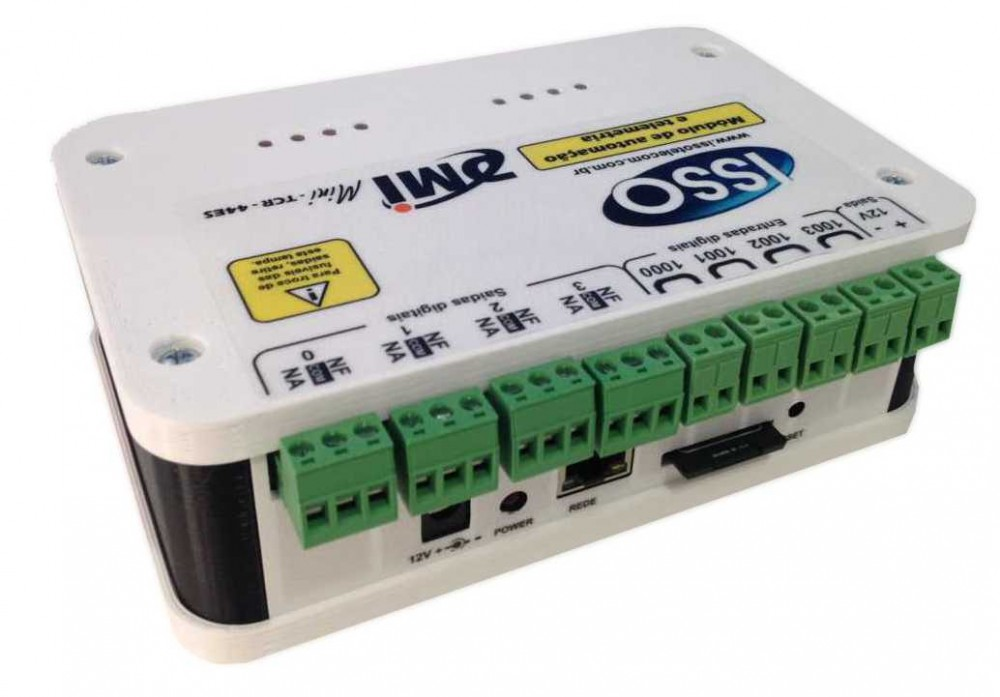
\includegraphics[width=\textwidth]{pictures/2010.jpg}
	\end{center}
	\fonte{\autocite{Isso44es}}
\end{figure}

Outro dispositivo, denominado Bridge101A, mostrado na \autoref{fig:2030}, fabricado pela empresa Madgetech foi encontrado, segundo a empresa é um data logger compacto que mede e armazena valores de tensões elétricas,
e é normalmente utilizado com extensômetros, células de carga e outras sensores de baixa tensão, e que o dispositivo é utilizado para calcular com precisão parâmetros de tensão, torque, deformação
e pressão ao longo do tempo. \autocite{Bridge101A}

\begin{figure}[htb]
	\caption{\label{fig:2030} Dispositivo Bridge101A}
	\begin{center}
		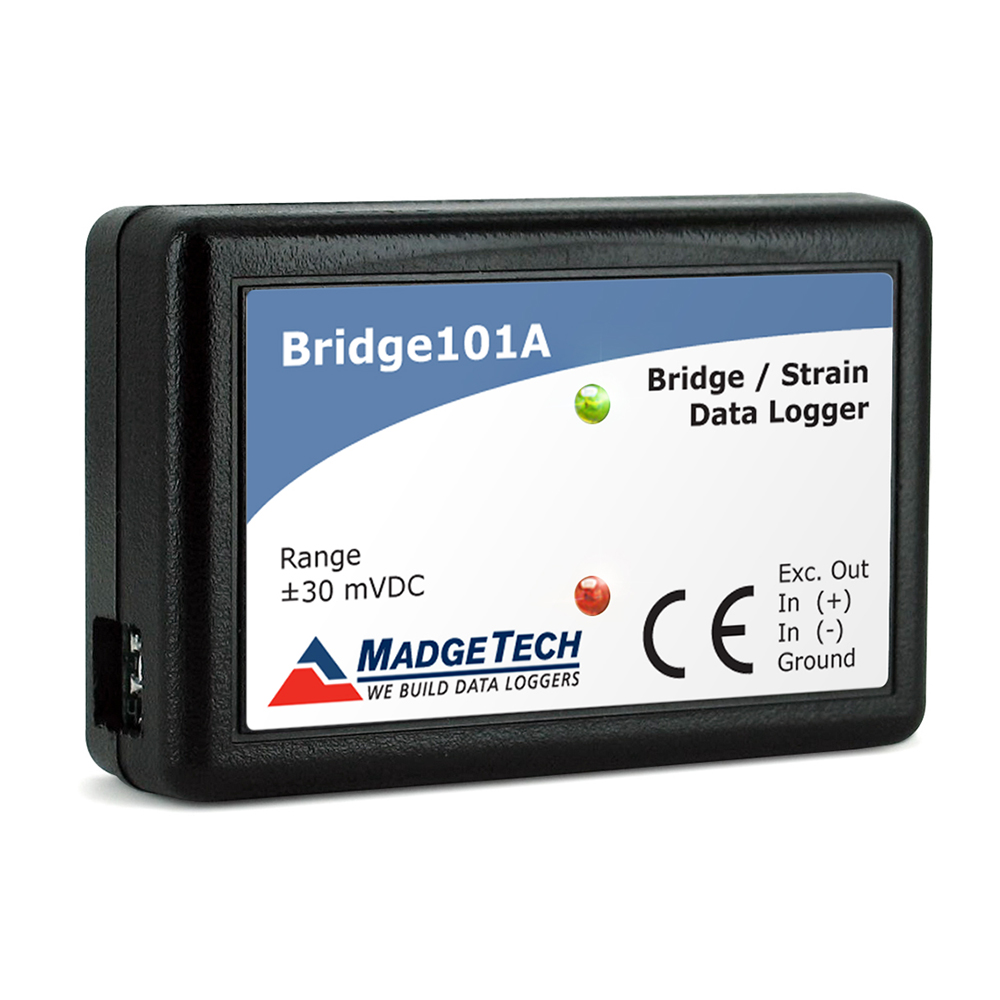
\includegraphics[width=\textwidth]{pictures/2030.jpg}
	\end{center}
	\fonte{\autocite{Bridge101A}}
\end{figure}

A \autoref{tab:Banchmarking} mostra uma comparação entre os dados de utilização obtidos pela documentação dos dois dispositivos previamente apresentados.

\begin{table}[!ht]
    \caption{Benchmarking entre dispositivos encontrados}
    \label{tab:Banchmarking}
    \centering
    \resizebox{\linewidth}{!}{%
        \begin{tabular}{ l | c c r } \toprule
         			  & Isso DMI TCR 44es & Isso DMI TCR 88es & Madgetech Bridge101A \\
			\midrule
			Dimensões & 124x117x55mm & 190x117x55mm & 36x64x16mm \\
			Comunicação com PC & Conexão Ethernet & Conexão Ethernet & Conexão USB \\
%			Interface com o usuário & Software próprio & Software próprio & Software próprio \\
%			Programação & Software próprio & Software próprio & Software próprio \\
			Taxa de leitura & Não disponiblizado & Não disponiblizado & $\SI{4}hz$ \\
			Faixa de tensão de leitura & Não disponiblizado & Não disponiblizado & $\SI{\pm 30}{\mV}$ \\
			Faixa de preço & R\$1100,00 & R\$1300,00 & R\$2800,00 \\
            \bottomrule
        \end{tabular}}
\fonte{O autor 2022}
\end{table}

Dentre os valores apresentados na tabela fica claro os altos preços envolvidos em qualquer aplicação que necessite a utilização desse tipo de dispositivo.
Muitos deles necessitam ainda de programas para programação e utilização proprietários e que ainda tem custos adicionais para utilização.
O dispositivo desenvolvido neste trabalho tem como objetivo um preço consideravelmente menor que os analisados e programável e utilizável utilizando tecnologias gratuitas
e de código aberto.

Uma possível aplicação mais específica de um produto semelhante aos pesquisados seria um dispositivo que possibilite a telemetria direta de cargas de torque presentes em
eixos de tração durante seu funcionamento, para isso seria necessário que o dispositivo fosse desenvolvido voltado para esse tipo de aplicação, a falta de um dispositivo
desse tipo disponível no mercado levou ao autor elaborar uma pesquisa científica focado em encontrar dispositivos desenvolvidos semelhantes a ideia.


\subsection{Pesquisa científica}

Com o intuito de facilitar o desenvolvimento do dispositivo, foi realizada uma revisão sistemática de trabalhos científicos e acadêmicos disponíveis nas bases de dados Web of Science, Springer,
Sciencedirect e Google Scholar, utilizando como palavras-chave “Dynamic, Torque, Shaft, Sensor, Strain, Gauge”, os principais obtidos são apresentados nessa subseção.

Um artigo desenvolvido por \autocite{Niedworok2014} relata o desenvolvimento e aplicação de um sistema de sensoriamento de torque em tempo real em um eixo cardan de um carro de mina utilizando a medição
da deformação utilizando extensômetro com transferência dos dados via radiofrequência, o trabalho também indica que o posicionamento do sensor necessita estar em contato com a superfície de maior deformação do componente,
o autor realiza uma análise por elementos finitos para encontrar esse local. O artigo também aponta que o sinal vindo do sensor deve ser ampliado utilizando uma ponte de Wheatstone para conseguir ter a instrumentação
correta da grandeza. O artigo mostrou resultados satisfatórios e não discutiu sobre ruídos e imprecisões presentes nos dados obtidos.

\autocite{Nurprasetio2018} desenvolve, em seu trabalho, um sistema de medição para veículos terrestres, aplicado em uma bancada de testes que simula o estado de veículos terrestres em operação, o sistema
utiliza um microprocessador Arduino nano de fácil acesso e baixo custo. Os dados são transmitidos via comunicação bluetooth. O artigo também ilustra o processo de calibração do dispositivo feito antes do teste dinâmico,
assim como no trabalho anterior, também é enfatizada a necessidade das metodologias de instrumentação do sinal vindo do extensômetro. Seus resultados também se mostraram promissores, porém o autor indica que é necessário
a remoção dos ruídos de medição, o que segundo ele será endereçado em um trabalho futuro.

\autocite{Gharghan2017} compara um sistema de medição similar ao dos dois trabalhos prévios com um sistema de medição de torque em tempo real de alto custo utilizado por ciclistas profissionais no pedivela.
O artigo introduz a tecnologia de transmissão de dados Zigbee, que consegue transmitir dados a um baixo consumo energético. Após a obtenção dos dados, o autor utiliza as ferramentas de análise estatística de Bland-Altman
e porcentagem de erro médio absoluto para a validação do sistema.

\autocite{Silva2017} compara os dados de um sistema semelhante aos anteriores com resultados de análises de modelo matemático analítico e análise por elementos finitos aplicados em bancadas de viga engastada com carga
na ponta e de torque aplicado em um eixo com um dos lados travados, diferente dos trabalhos anteriores, este possui uma seção com o desenvolvimento das equações dos modelos utilizados, e assim como os artigos anteriores
foram encontrados resultados satisfatórios.

A ideia inicial da concepção do produto seria o do desenvolvimento de um dispositivo que obtivesse os valores de torque em um eixo em tempo real. Para que fosse possível solucionar tal problema, o dispositivo teria que
obter os dados de tensão dos pólos de uma ponte de wheatstone, com um extensômetro montado a um eixo sob torque e transmitir os dados obtidos via conexão sem fio em tempo real a um computador. O projeto inicial do
dispositivo é mostrado na \autoref{fig:2029}.

\begin{figure}[htb]
	\caption{\label{fig:2029} Projeto inicial do dispositivo}
	\begin{center}
		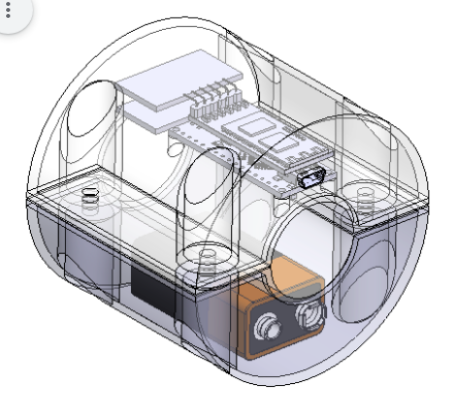
\includegraphics[width=\textwidth]{pictures/2029.png}
	\end{center}
	\fonte{O autor 2022}
\end{figure}

O conceito é composto por uma placa de desenvolvimento Arduino, que controla um amplificador de sinal que por si obtém os dados de tensão de uma ponte de wheatstone. Os dados obtidos pela ponte de wheatstone então
são transmitidos utilizando um módulo bluetooth HC-05. O custo total desses dois componentes é baixo, e um protótipo de dispositivo pode ser montado por aproximadamente R$150,00, desconsiderando os componentes de
encapsulamento. O projeto informacional é iniciado considerando este conceito como a ideia inicial do produto.

\section{Projeto informacional}

Uma vez que a ideia inicial do produto é caracterizada pelo grande potencial de ser de baixo custo e de ser consideravelmente compacto em relação aos outros produtos
encontrados no mercado, pode-se traçar uma estratégia de definição de público alvo, o que facilita as tomadas de decisão durante o desenvolvimento do produto.
Dentre os possíveis públicos que são beneficiados pelas características do produto que será desenvolvido, as equipes de competição Baja SAE foram
escolhidas como público alvo para guiar o desenvolvimento do dispositivo, uma vez que o baixo custo, baixas dimensões e flexibilidade de aplicação são características
desejadas para utilização nesses grupos.

Foi elaborado um formulário eletrônico que apresenta a ideia do conceito de funcionamento de um dispositivo para sensoriar dados de torque em tempo real. No formulário
são apresentadas duas perguntas iniciais, que avaliam a importância da obtenção desse tipo de dado e a importância de serem obtidas em tempo real, além das duas perguntas
iniciais, são apresentados os seguintes tópicos sobre a necessidade do produto em desenvolvimento de:

\begin{alineas}

	\item Qual sua opinião sobre a importância da obtenção de dados de torque, potência e rotação do sistema de propulsão durante a utilização?;
	\item Qual sua opinião sobre o recebimento a distância e ilustração desses dados em tempo real?;
	\item Capacidade de gravação/armazenamento de dados;
	\item Ser de baixo preço;
	\item Ser compacto;
	\item Ser leve;
	\item Suportar grande variação da faixa de torque;
	\item Ser a prova de água, fluidos, poeira, lama, etc;
	\item Ser resistente a impactos;
	\item Ser de fácil utilização e montagem;
	\item Ser de fácil manutenção;
	\item Possuir bateria de longa duração (duração da prova mais longa);
	\item Possuir disjuntor/botão de liga/desliga;

\end{alineas}

Todas as perguntas e tópicos foram respondidos pela seleção de uma nota de 1 a 5 para cada questão, onde o valor 1 significa que o requisito listado é de baixa importância e
o valor 5 é de extrema importância. As respostas do formulário são avaliadas pela análise do valor médio obtido pelos valores respondidos. Foram obtidas as respostas de 8
membros de diferentes equipes de competição. Os resultados são mostrados na \autoref{tab:resultpesquisa}.

\begin{table}[!ht]
    \caption{Resultado pesquisa de mercado}
    \label{tab:resultpesquisa}
    \centering
    \resizebox{\textwidth}{!}{%
        \begin{tabular}{ l | r } \toprule
         	Pergunta/Requisito & Importância \\
			\midrule
			 Importância de obtenção dos dados & 4.875 \\
			 Importancia de obtenção em tempo real & 3.875 \\
			 Ser de baixo preço & 3.625\\
			 Ser compacto & 3.875\\
			 Ser leve & 3.75\\
			 Suportar grande variação da faixa de torque & 4.125\\
			 Ser a prova de água, fluidos, poeira, lama, etc & 4.75\\
			 Ser resistente a impactos & 4\\
			 Ser de fácil utilização e montagem & 3.375\\
			 Ser de fácil manutenção & 3.75\\
			 Possuir bateria de longa duração & 4.25\\
			 Possuir botão de liga/desliga & 3.375\\
			 Capacidade de gravação de dados & 4.125\\
            \bottomrule
        \end{tabular}}
\fonte{O autor 2022}
\end{table}

Com as respostas do formulário de pesquisa do público alvo, pode ser elaborada uma matriz de listagem de atributos, que serve para mapear quais funcionalidades produto deve ter para atender cada um dos requisitos
do produto, e quais sistemas necessários para garantir as funcionalidades listadas, a matriz é mostrada na \autoref{fig:2031}.

\begin{figure}[htb]
	\caption{\label{fig:2031} Matriz de listagem de atributos}
	\begin{center}
		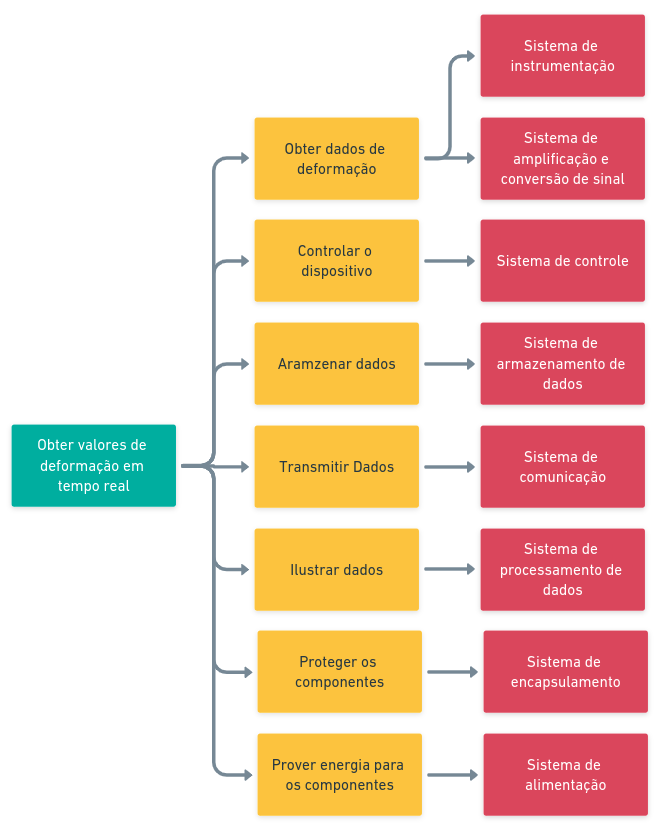
\includegraphics[width=\textwidth]{pictures/2031.png}
	\end{center}
	\fonte{O autor 2022}
\end{figure}

Com os dados de avaliação quantitativa dos requisitos do produto obtidas pela pesquisa com o público alvo e os dados de requisitos dos sistemas necessários para atender os requisitos do diagrama de listagem de
atributos pode-se então elaborar uma matriz de avaliação de qualidade, chamada de matriz QFD. Essa matriz mostra as relações entre os requisitos do cliente com as características desejadas do produto,
com a finalidade de apontar quais as qualidades devem ser priorizadas na etapa de desenvolvimento do projeto.

\begin{figure}[htb]
	\caption{\label{fig:2032} Matriz QFD}
	\begin{center}
		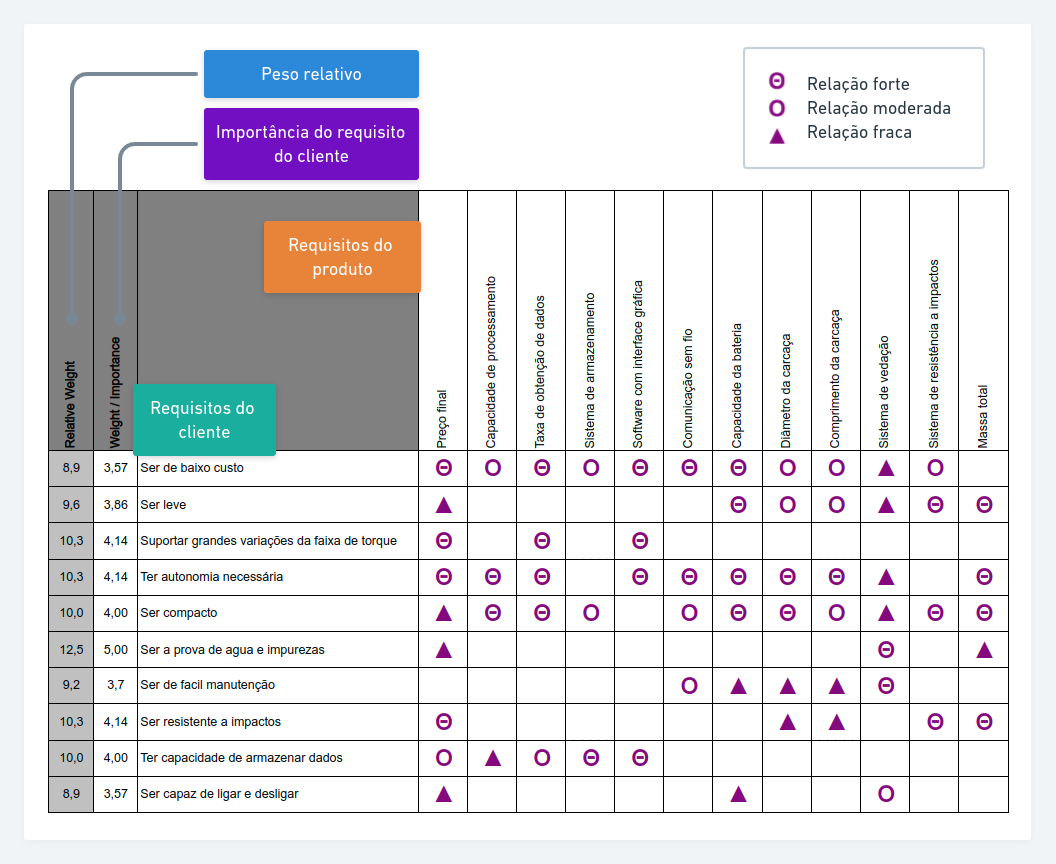
\includegraphics[width=\textwidth]{pictures/2032.png}
	\end{center}
	\fonte{O autor 2022}
\end{figure}

O resultado dos calculos de prioridade realizado pela matriz QFD são apresentados na \autoref{tab:resultqfd}.

\begin{table}[!ht]
    \caption{Prioridade dos requisitos definidos pela matriz QFD}
    \label{tab:resultqfd}
    \centering
    \resizebox{\textwidth}{!}{%
        \begin{tabular}{ l | r } \toprule
         	Pergunta/Requisito & Importância \\
			\midrule
			req1 & 4.875 \\
			req2 & 3.875 \\
			req3 & 3.625 \\
			req4 & 3.875 \\
			req5 & 3.75 \\
            \bottomrule
        \end{tabular}}
\fonte{O autor 2022}\
\end{table}

%Utilizando o modelo de QFD também é realizada uma comparação do conceito do produto que será desenvolvido com as opções disponíveis no mercado previamente mencionadas, com a finalidade de indicar as vantagens de se utilizar o conceito desenvolvido em relação aos outros modelos disponíveis.

\section{Projeto conceitual}



\section{Projeto detalhado}

\section{Projeto preliminar}

\subsection[]{Montagem do dispositivo}

\begin{table}[!ht]
    \caption{Características de ganho para o ADS1115}
    \label{tab:ads1115modes}
    \centering
    \resizebox{\textwidth}{!}{%
        \begin{tabular}{ l | c c r } \toprule
         	Ganho & Faixa de leitura & Resolução \\
			\midrule
			 2/3x & ${\pm 6.144}V$ & $1bit$ = ${0.1875}{m}V$ \\
			 1x & ${\pm 4.096}V$ & $1bit$ = ${0.125}{m}V$ \\
			 2x & ${\pm 2.048}V$ & $1bit$ = ${0.0625}{m}V$ \\
			 4x & ${\pm 1.024}V$ & $1bit$ = ${0.03125}{m}V$ \\
			 8x & ${\pm 0.512}V$ & $1bit$ = ${0.015625}{m}V$ \\
			 16x & ${\pm 0.256}V$ & $1bit$ = ${0.0078125}{m}V$ \\
            \bottomrule
        \end{tabular}}
\fonte{O autor 2022}
\end{table}

\subsection[]{Desenvolvimento do software}

\begin{figure}[htb]
	\caption{\label{fig:2034} Objeto SerialDevice}
	\begin{center}
		\includegraphics[width=\textwidth]{pictures/2034.png}
	\end{center}
	\fonte{O autor 2022}
\end{figure}


\begin{figure}[htb]
	\caption{\label{fig:2035} Interface gráfica}
	\begin{center}
		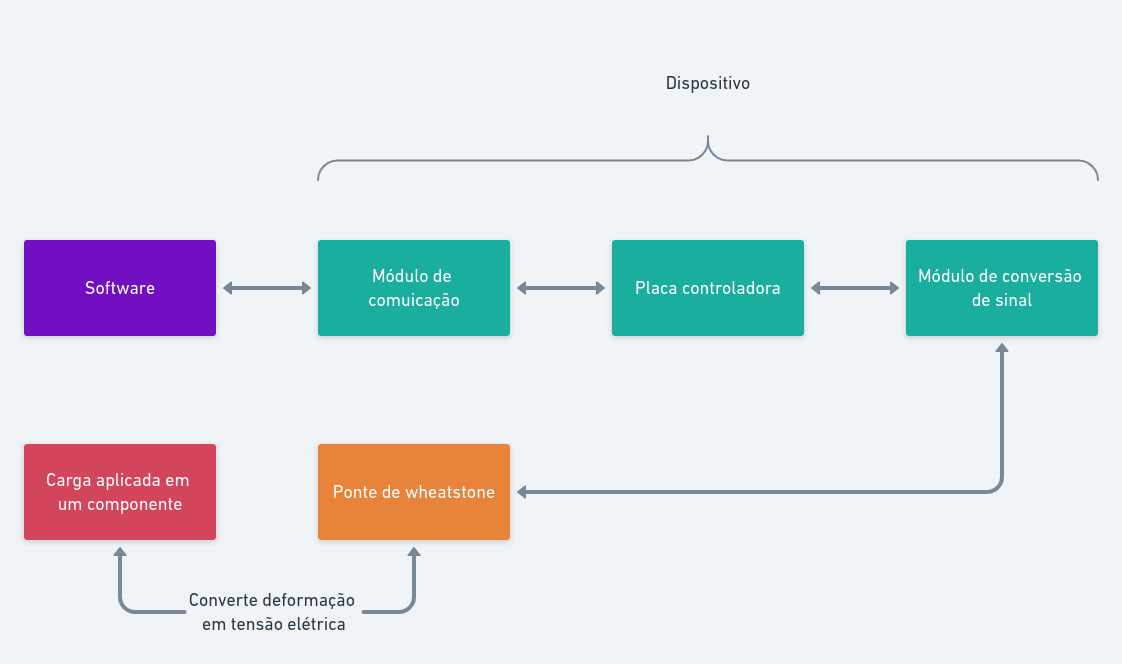
\includegraphics[width=\textwidth]{pictures/2035.png}
	\end{center}
	\fonte{O autor 2022}
\end{figure}


\begin{lstlisting}[language=Python,caption={[Objeto SerialDevice]{SerialDevice}}]
class SerialDevice:
    """
    Creates a serial connection device object
    """
    from serial import Serial

    def __init__(self, port, baudrate, delay_time):
        self.serial_object = self.Serial(port=port, baudrate=baudrate, timeout=1)
        self.delay_time = float(delay_time) * 1e-3

    def read_line(self):
        """returns the last line of data sent by the device"""
        self.serial_object.flushInput()
        data = self.serial_object.readline()
        return data

    def read_samples(self, n_of_samples):
        """returns a number of data lines given a sample size"""
        current_sample = 0
        data = []
        while current_sample < n_of_samples:
            data.append(self.read_line())
            current_sample += 1
        return data
\end{lstlisting}


\begin{lstlisting}[language=Python,caption={[Objeto SerialDevice]{SerialDevice}}]
class SerialDevice:
    """
    Creates a serial connection device object
    """
    from serial import Serial

    def __init__(self, port, baudrate, delay_time):
        self.serial_object = self.Serial(port=port, baudrate=baudrate, timeout=1)
        self.delay_time = float(delay_time) * 1e-3

    def read_line(self):
        """returns the last line of data sent by the device"""
        self.serial_object.flushInput()
        data = self.serial_object.readline()
        return data

    def read_samples(self, n_of_samples):
        """returns a number of data lines given a sample size"""
        current_sample = 0
        data = []
        while current_sample < n_of_samples:
            data.append(self.read_line())
            current_sample += 1
        return data
\end{lstlisting}



\section{Validação do protótipo}

A metodologia de execução do experimento para validar o funcionamento do protótipo desenvolvido segue a mesma metodologia do experimento realizado no trabalho de conclusão
de curso de \autocite{Minela2017}, uma introdução aos principais tópicos dessa metodologia e eventuais diferenças entre os dispositivos utilizados nos dois trabalhos para cada tópico é feita nessa seção.

Os ensaios realizados envolvem a leitura de extensômetros colados em corpos de prova sobre ação de cargas específicas. Um dispositivo de análise de cargas de flexão e
um para cargas em torção foram desenvolvidos e produzidos por \autocite{Minela2017}, os mesmos dispositivos foram utilizados para este trabalho.

\subsection{Dispositivo para ensaio de flexão}

O dispositivo para realizar o ensaio de flexão é composto por uma viga de seção retangular de $20mm$ de largura por $2mm$ de espessura, que mede $200mm$
de comprimento e é de uma liga desconhecida de alumínio, e uma base projetada e fabricada em aço 1020 para fixar a viga em uma situação de engaste na viga.
A imagem mostra o projeto do dispositivo desenvolvido por \autocite{Minela2017}.

\begin{figure}[htb]
	\caption{\label{fig:2040} Dispositivo de ensaio de flexão}
	\begin{center}
		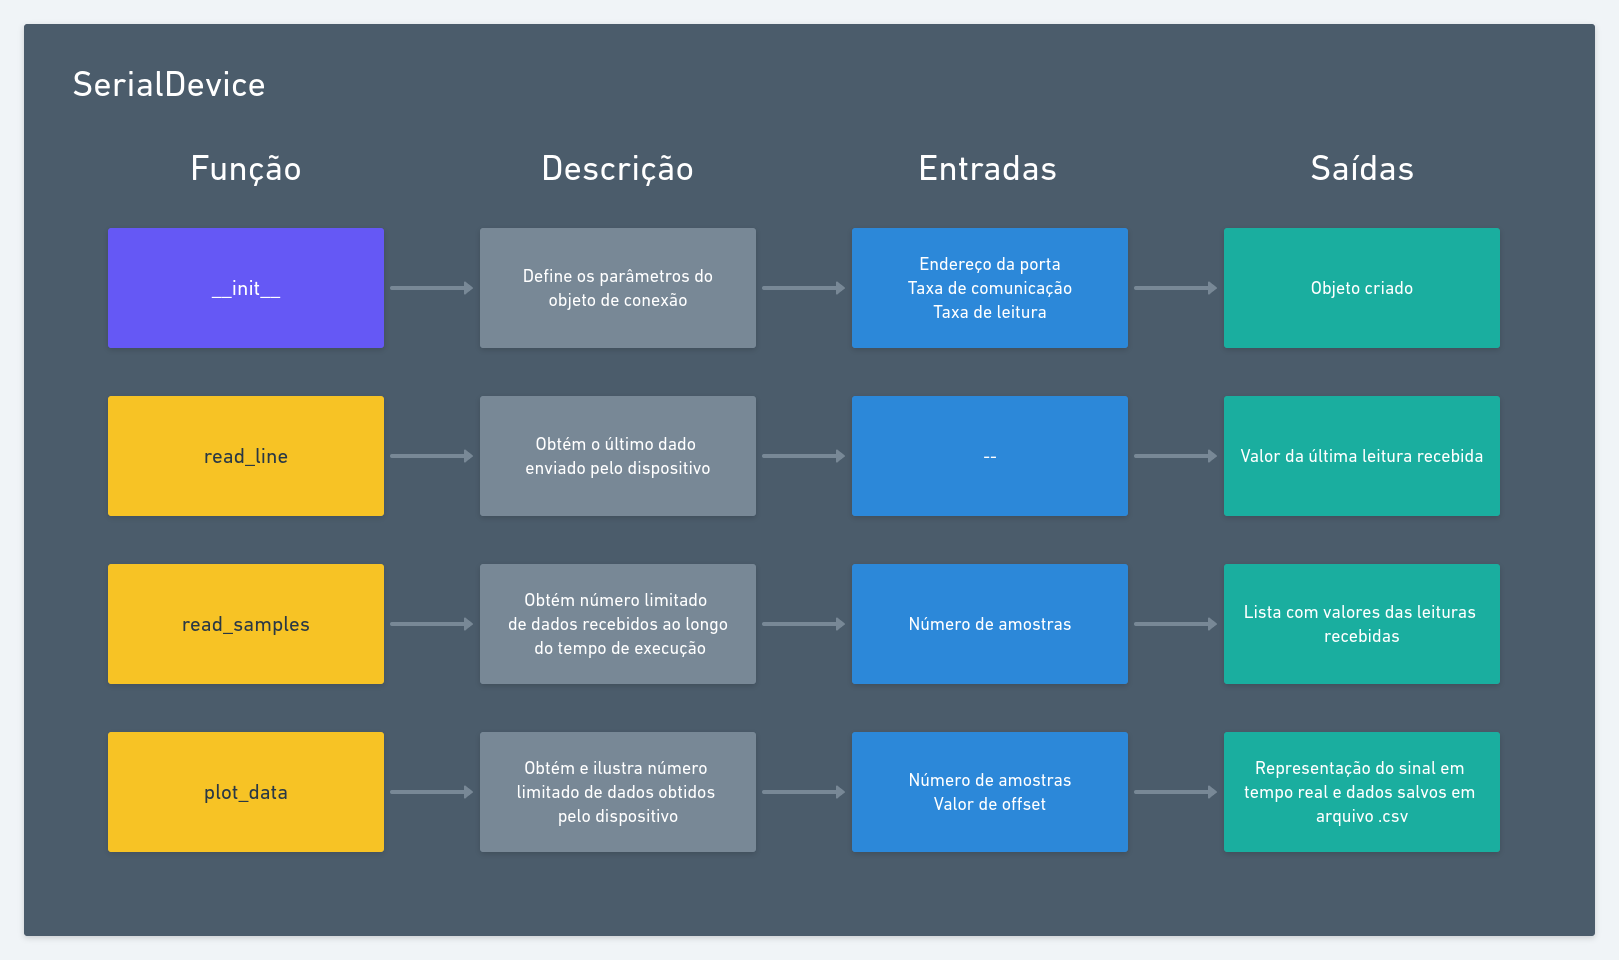
\includegraphics[width=\textwidth]{pictures/2040.png}
	\end{center}
	\fonte{\autocite{Minela2017}}
\end{figure}

Na viga é colado um extensômetro unidimensional para obter os dados de deformação, as propriedades do extensômetro utilizado são mostradas na
\autoref{tab:PropriedadesExtensometro}.

\begin{table}[htb]
\caption[]{Propriedades do extensômetro colado ao dispositivo de flexão}
\label{tab:PropriedadesExtensometro}
\resizebox{\textwidth}{!}{%
\begin{tabular}{p{6.5cm}p{8cm}}
	\toprule
	Marca & Micro Measurements \textregistered \\
	Tipo de extensômetro & EA-06-250AF-120 \\
	Resistência Elétrica & ${120\pm 0.15\% \Omega}$ \\
	Factor de gage até ${75 ^\circ F}$ & ${2.025 \pm 0.5 \%}$ \\
	Comprimento & ${6.35} \mm$ \\
	Limite de têmperatura & ${-75\tccentigrade}$ á ${175\tccentigrade}$ para medições estáticas \\
	\bottomrule
\end{tabular}
}
\fonte{Adapdato de \autocite{Minela2017}}
\end{table}

As cargas são aplicadas na extremidade livre da viga a distância de 150mm entre o centro do extensômetro e o ponto de aplicação da carga.
Com a finalidade de se obter os valores de deformação causados pela aplicação de cada carga, cada trabalho utiliza-se de um sistema de medição diferente, apresentado
na seção seguinte.

\subsection{Sistemas de medição}

Tanto o sistema de medição utilizado em \autocite{Minela2017} quanto o utilizado para o desenvolvimento deste trabalho seguem o mesmo princípio de funcionamento.

\begin{figure}[htb]
	\caption{\label{fig:2050} Sistema de medição utilizado por \autocite{Minela2017}}
	\begin{center}
		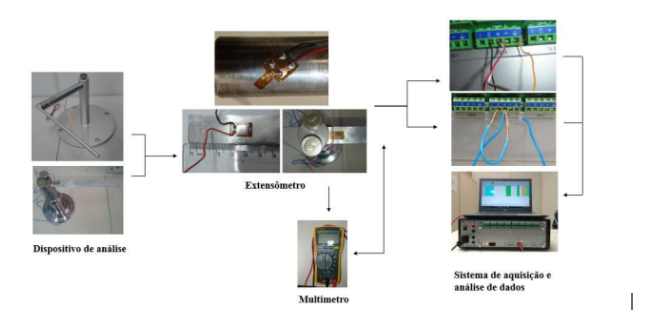
\includegraphics[width=\textwidth]{pictures/2050.png}
	\end{center}
	\fonte{\autocite{Minela2017}}
\end{figure}

O sistema de medição utilizado por \autocite{Minela2017} é composto por um dispositivo de obtenção de dados ADS2002, desenvolvido e fabricado pela LYNX Tecnologia,
que é conectado a um computador. O ADS2002 obtém os dados gerados pelo sensor e os envia ao computador via conexão ethernet.
O computador utiliza o software AQDados para conexão com o ADS2002, calibração e aferição dos extensômetros, e o softwre AqAnalysis para fazer o processamento dos sinais
e gerar relatórios de análise, ambos os programas são desenvolvidos pela fabricante do dispositivo de obtenção de dados.

\begin{figure}[htb]
	\caption{\label{fig:2060} Sistema de de medição utilizando o LINX ADS2002}
	\begin{center}
		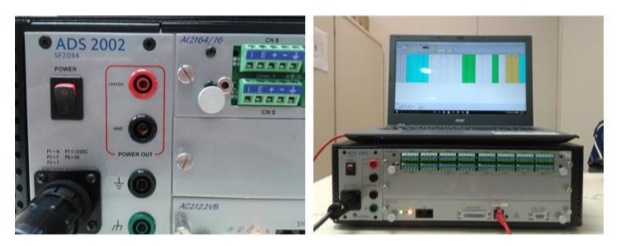
\includegraphics[width=\textwidth]{pictures/2060.png}
	\end{center}
	\fonte{\autocite{Minela2017}}
\end{figure}

A conexão entre o dispositivo de obtenção de dados e o extensômetro ocorre utilizando os terminais elétricos do canal específico de análise, o ADS2002 já possui,
integrado em si, os componentes elétricos do circuito da ponte de wheatstone para a instrumentação do sinal.
A calibração do extensômetro afim dos resultados serem mostrados como valores deformação, ao invés de tensões, é feita utilizando a \autoref{eq:Eq_270} que define um valor de
fator de engenharia em função do fator gage $FG$ da resistência média do extensômetro $RM$, resistência de calibração $RC$, que é disponibilizada pelo fabricante.

\begin{equation}\label{eq:Eq_270}%
\mbox{\fontsize{17.28}{21.6}\selectfont\( %
VE = \left ( \frac{1}{FG}\left ( \frac{RM}{RM + RC} \right ) \right )
\)} %
\end{equation}

\newline

O sistema de medição utilizando o protótipo desenvolvido pelo autor é feito pela conexão entre o controlador ESP 32 e o computador via o software desenvolvido em python
para realizar a transferência dos dados obtidos entre o controlador e o computador em tempo real.

\begin{figure}[htb]
	\caption{\label{fig:2070} Protótipo do dispositivo desenvolvido conectado com o extensometro no dispositivo de flexão}
	\begin{center}
		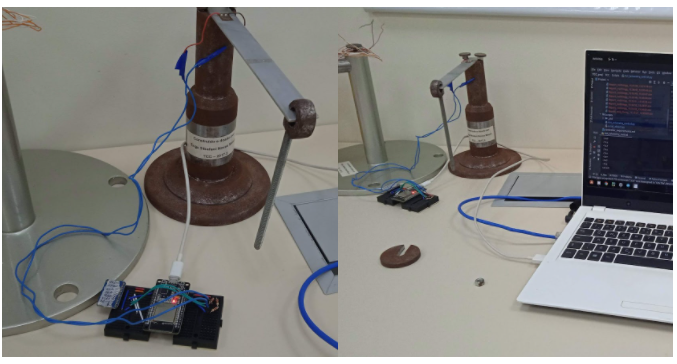
\includegraphics[width=\textwidth]{pictures/2070.png}
	\end{center}
	\fonte{O autor 2021}
\end{figure}

A calibração do dispositivo desenvolvido pelo autor é feita utilizando os sinais resultantes da aplicação de duas massas distintas conhecidas.
Os valores nominais obtidos nos sinais alimentam a \autoref{eq:Eq_280} que é utilizada para converter os valores discretos obtidos em bits pelo
amplificador de sinal para um valor de gradeza física desejado.

\begin{equation}\label{eq:Eq_280}%
\mbox{\fontsize{17.28}{21.6}\selectfont\( %
F(W) = \frac{output_{high}-output_{low}}{W_{high}-W_{low}}(W - W_{low}) + output_{low}
\)} %
\end{equation}

onde

$F(W)$: Função de calibração

$W$: Valor nominal do sinal

$W_{high}$: Carga de calibração de massa alta

$W_{low}$: Carga de calibração de massa baixa

$output_{high}$: Valor nominal do sinal obtido pela aplicação da carga alta

$output_{high}$: Valor nominal do sinal obtido pela aplicação da carga baixa

\hfill

A calibração ocorre por um método automatizado implementado no software de comunicação entre o controlador e o computador.
Após calibrado, o dados são mostrados como os valores de grandeza física calibrada.

\subsection{Cargas aplicadas}

\autocite{Minela2017} utiliza pesos com massas pré definidas apoiadas utilizando um fuso de fixação para aplicação das cargas no ponto “F” no dispositivo, mostrado na figura.
Dentre as massas utilizadas por \autocite{Minela2017} duas não foram localizadas pelo autor deste trabalho, com a finalidade de poder se obter resultados que se possam fazer
comparações diretas entre os trabalhos foram substituidas as massas não encontradas por massas semelhantes.

Todos os valores de massa dos pesos utilizados foram obtidos novamente pelo autor utilizando o valor médio de três leituras obtidas por uma balança de precisão disponibilizada pelo laboratório de metrologia
da UFSC Joinville. Os valores obtidos são apresentados na \autoref{tab:MassasUtilizadas}.

\begin{table}[!ht]
    \caption{Valores de massas utilizadas para aplicação das cargas nos dispositivos de flexão e torção}
    \label{tab:MassasUtilizadas}
    \centering
    \resizebox{\linewidth}{!}$ \\
            Fuso & $\SI{48.63}{\g}$ & $\SI{48.78}{\g}$ & $\SI{0.31}{\%}$ \\
            Peso 1 & $\SI{86.73}{\g}$ & $\SI{99.68}{\g}$ & $\SI{12.99}{\%}$ \\
            Peso 2 & $\SI{198.38}{\g}$ & $\SI{198.36}{\g}$ & $\SI{0.01}{\%}$ \\
            Peso 3 & $\SI{997.13}{\g}$ & $\SI{997.3}{\g}$ & $\SI{0.02}{\%}$ \\
            Peso 4 & $\SI{497.66}{\g}$ &$\SI{497.69}{\g}$ & $\SI{0.02}{\%}$ \\
            Peso 5 & $\SI{495.25}{\g}$ & $\SI{496.22}{\g}$ & $\SI{0.20}{\%}$ \\
            \bottomrule
        \end{tabular}}
\fonte{O autor 2022}
\end{table}

As massas da porca e do “peso 1” utilizados em \autocite{Minela2017} variam de forma considerável em relação aos pesos utilizados neste trabalho, então para todas as comparações diretas de
resultados experimentais obtidos entre os dois trabalhos deve ser aplicados fatores de correção de 11.42g para a porca e 12.95g para o “peso 1”.

O método de aplicação de cargas é caracterizado pela aplicação na extremidade livre da viga das massas utilizando o fuso como suporte, a Figura mostra a viga de aluminio defletida pela aplicação da carga do "peso 3".

\begin{figure}[htb]
	\caption{\label{fig:2080} Aplicaçao do 'peso 3' no dispositivo de flexão}
	\begin{center}
		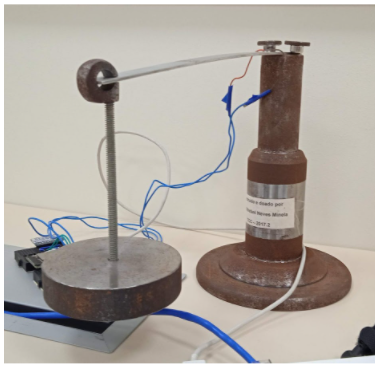
\includegraphics[width=\textwidth]{pictures/2080.png}
	\end{center}
	\fonte{O autor 2021}
\end{figure}

Na extremidade da viga encontra-se uma demarcação para auxiliar o posicionamento do apoio do fuso e as cargas são aplicadas de maneira cuidadosa de modo que não sejam geradas forças de impulso na viga.
O sistema de medição obtem valores em bits proporcionais a carga aplicada no experimento.

Os valores obtidos em bits são posteriormente convertidos em valores de carga, ou de deformação utilizando uma função de transferencia obtida pelo método de calibração.
